
\resetcounters

\markboth{Bulgarelli et al.}{AGILE-GRID Science Alert Monitoring System }

\title{\ssindex{observatories!space-based!AGILE}AGILE/\ssindex{instruments!individual!GRID}GRID Science Alert Monitoring System: The Workflow and the Crab Flare Case}
\author{A.~Bulgarelli,$^1$ M.~Trifoglio,$^1$ F.~Gianotti,$^1$ 
M.~Tavani,$^2$ V.~Conforti,$^1$ and N.~Parmiggiani$^3$
\affil{$^1$National Institute for Astrophysics - IASF Bologna, Italy}
\affil{$^2$National Institute for Astrophysics - IAPS Roma, Italy}
\affil{$^3$University of Modena and Reggio Emilia}}

\aindex{Bulgarelli, A.}
\aindex{Trifoglio, M.}
\aindex{Gianotti, F.}
\aindex{Tavani, M.}
\aindex{Conforti, V.}
\aindex{Parmiggiani, N.}

\begin{abstract}
During the first five years of the \ssindex{observatories!space-based!AGILE}AGILE mission we have observed many \ssindex{astronomy!gamma-ray}gamma-ray \ssindex{astronomy!transients}transients of\ssindex{astronomy!Galactic} Galactic and \ssindex{astronomy!extragalactic}extragalactic origin. A fast reaction to unexpected \ssindex{astronomy!transients}transient events is a crucial part of the \ssindex{observatories!space-based!AGILE}AGILE monitoring program, because the follow-up of astrophysical \ssindex{astronomy!transients}transients is a key point for this space mission. We present the \ssindex{data!management!workflows}workflow and the software developed by the \ssindex{observatories!space-based!AGILE}AGILE Team to perform the \ssindex{software!automatic detection}automatic analysis  for the detection of \ssindex{astronomy!gamma-ray}gamma-ray \ssindex{astronomy!transients}transients. In addition, an App for \ssindex{computing!mobile!iPhone}iPhone will be released enabling the  Team to access the monitoring system through mobile phones. In 2010 September the science alert monitoring system presented in this paper recorded a \ssindex{astronomy!transients}transient phenomena from the Crab Nebula, generating an automated alert sent via email and SMS two hours after the end of an \ssindex{observatories!space-based!AGILE}AGILE satellite orbit, i.e. two hours after the Crab flare itself: for this discovery \ssindex{observatories!space-based!AGILE}AGILE won the 2012 Bruno Rossi prize. The design of this alert system is maximized to reach the maximum speed, and in this, as in many other cases, \ssindex{observatories!space-based!AGILE}AGILE has demonstrated that the reaction speed of the monitoring system is crucial for the scientific return of the mission. 
\end{abstract}

\section{Introduction}
The search for \ssindex{astronomy!gamma-ray}$\gamma$-ray \ssindex{astronomy!transients}transients (Galactic and \ssindex{astronomy!extragalactic}extragalactic) detectable on timescales of 1-2 days is one of the major activities performed by the AGILE Collaboration. Quick reaction times allow us to focus on \ssindex{astronomy!transients}transient events detected by \ssindex{observatories!space-based!AGILE}AGILE(Astrorivelatore Gamma ad Immagini LEggero - Light Imager for Gamma-ray Astrophysics) in the MeV-GeV energy range. Serendipitous \ssindex{astronomy!transients}transient discoveries during the \ssindex{observatories!space-based!AGILE}AGILE observation is possible given the large field of view and the \ssindex{observatories!space-based!AGILE}AGILE sensitivity. The \ssindex{observatories!space-based!AGILE}AGILE quick-look Science Alert Monitoring system  is a software and \ssindex{computers!hardware}hardware automated analysis system developed and used by AGILE team for alert generation of flares from astrophysical sources.

\ssindex{observatories!space-based!AGILE}AGILE is a scientific mission of the Italian Space Agency (ASI) launched on 2007 April 23 \citep{Tavani:2009ht}. The Gamma-Ray Imaging Detector (\ssindex{instruments!individual!GRID}GRID) for observations in the 30 MeV-50 GeV \ssindex{astronomy!gamma-ray}$\gamma$ energy range works with a very large fields of view (FOV) of more than 120 degrees across, i.e., 2.5 sr. The \ssindex{observatories!space-based!AGILE}AGILE orbital characteristics (quasi-equatorial with an inclination angle of 2.5 degrees and average 530 km altitude) are optimal for low-background  \ssindex{astronomy!gamma-ray}$\gamma$-ray observations. Each orbit last about 96 minutes. From 2009 Nov the \ssindex{observatories!space-based!AGILE}AGILE \ssindex{astronomy!gamma-ray}$\gamma$-ray observations of the sky are operated  with the satellite operating in "spinning mode" (the satellite axis sweeps an entire circle in the sky in approximately 7 min) with a typical accumulating pattern (see Figure~\ref{fig_fov}).            

The orbital characteristics, the large FOV and the operating modes had a great impact on the design of the science monitoring system and one of the key software requirements of the system was that the data processing should be completed within the next orbit to avoid or reduce backlog. This operating mode has required two different designs of the science alert monitoring system. In addition, an evaluation of the maximum likelihood method (the analysis method used by this system) for detecting short-term variability of AGILE \ssindex{astronomy!gamma-ray}$\gamma$-ray sources is a key point of this monitoring system \citep{Bulgarelli:2012ds}.
                   
\begin{figure}[t]
\centering
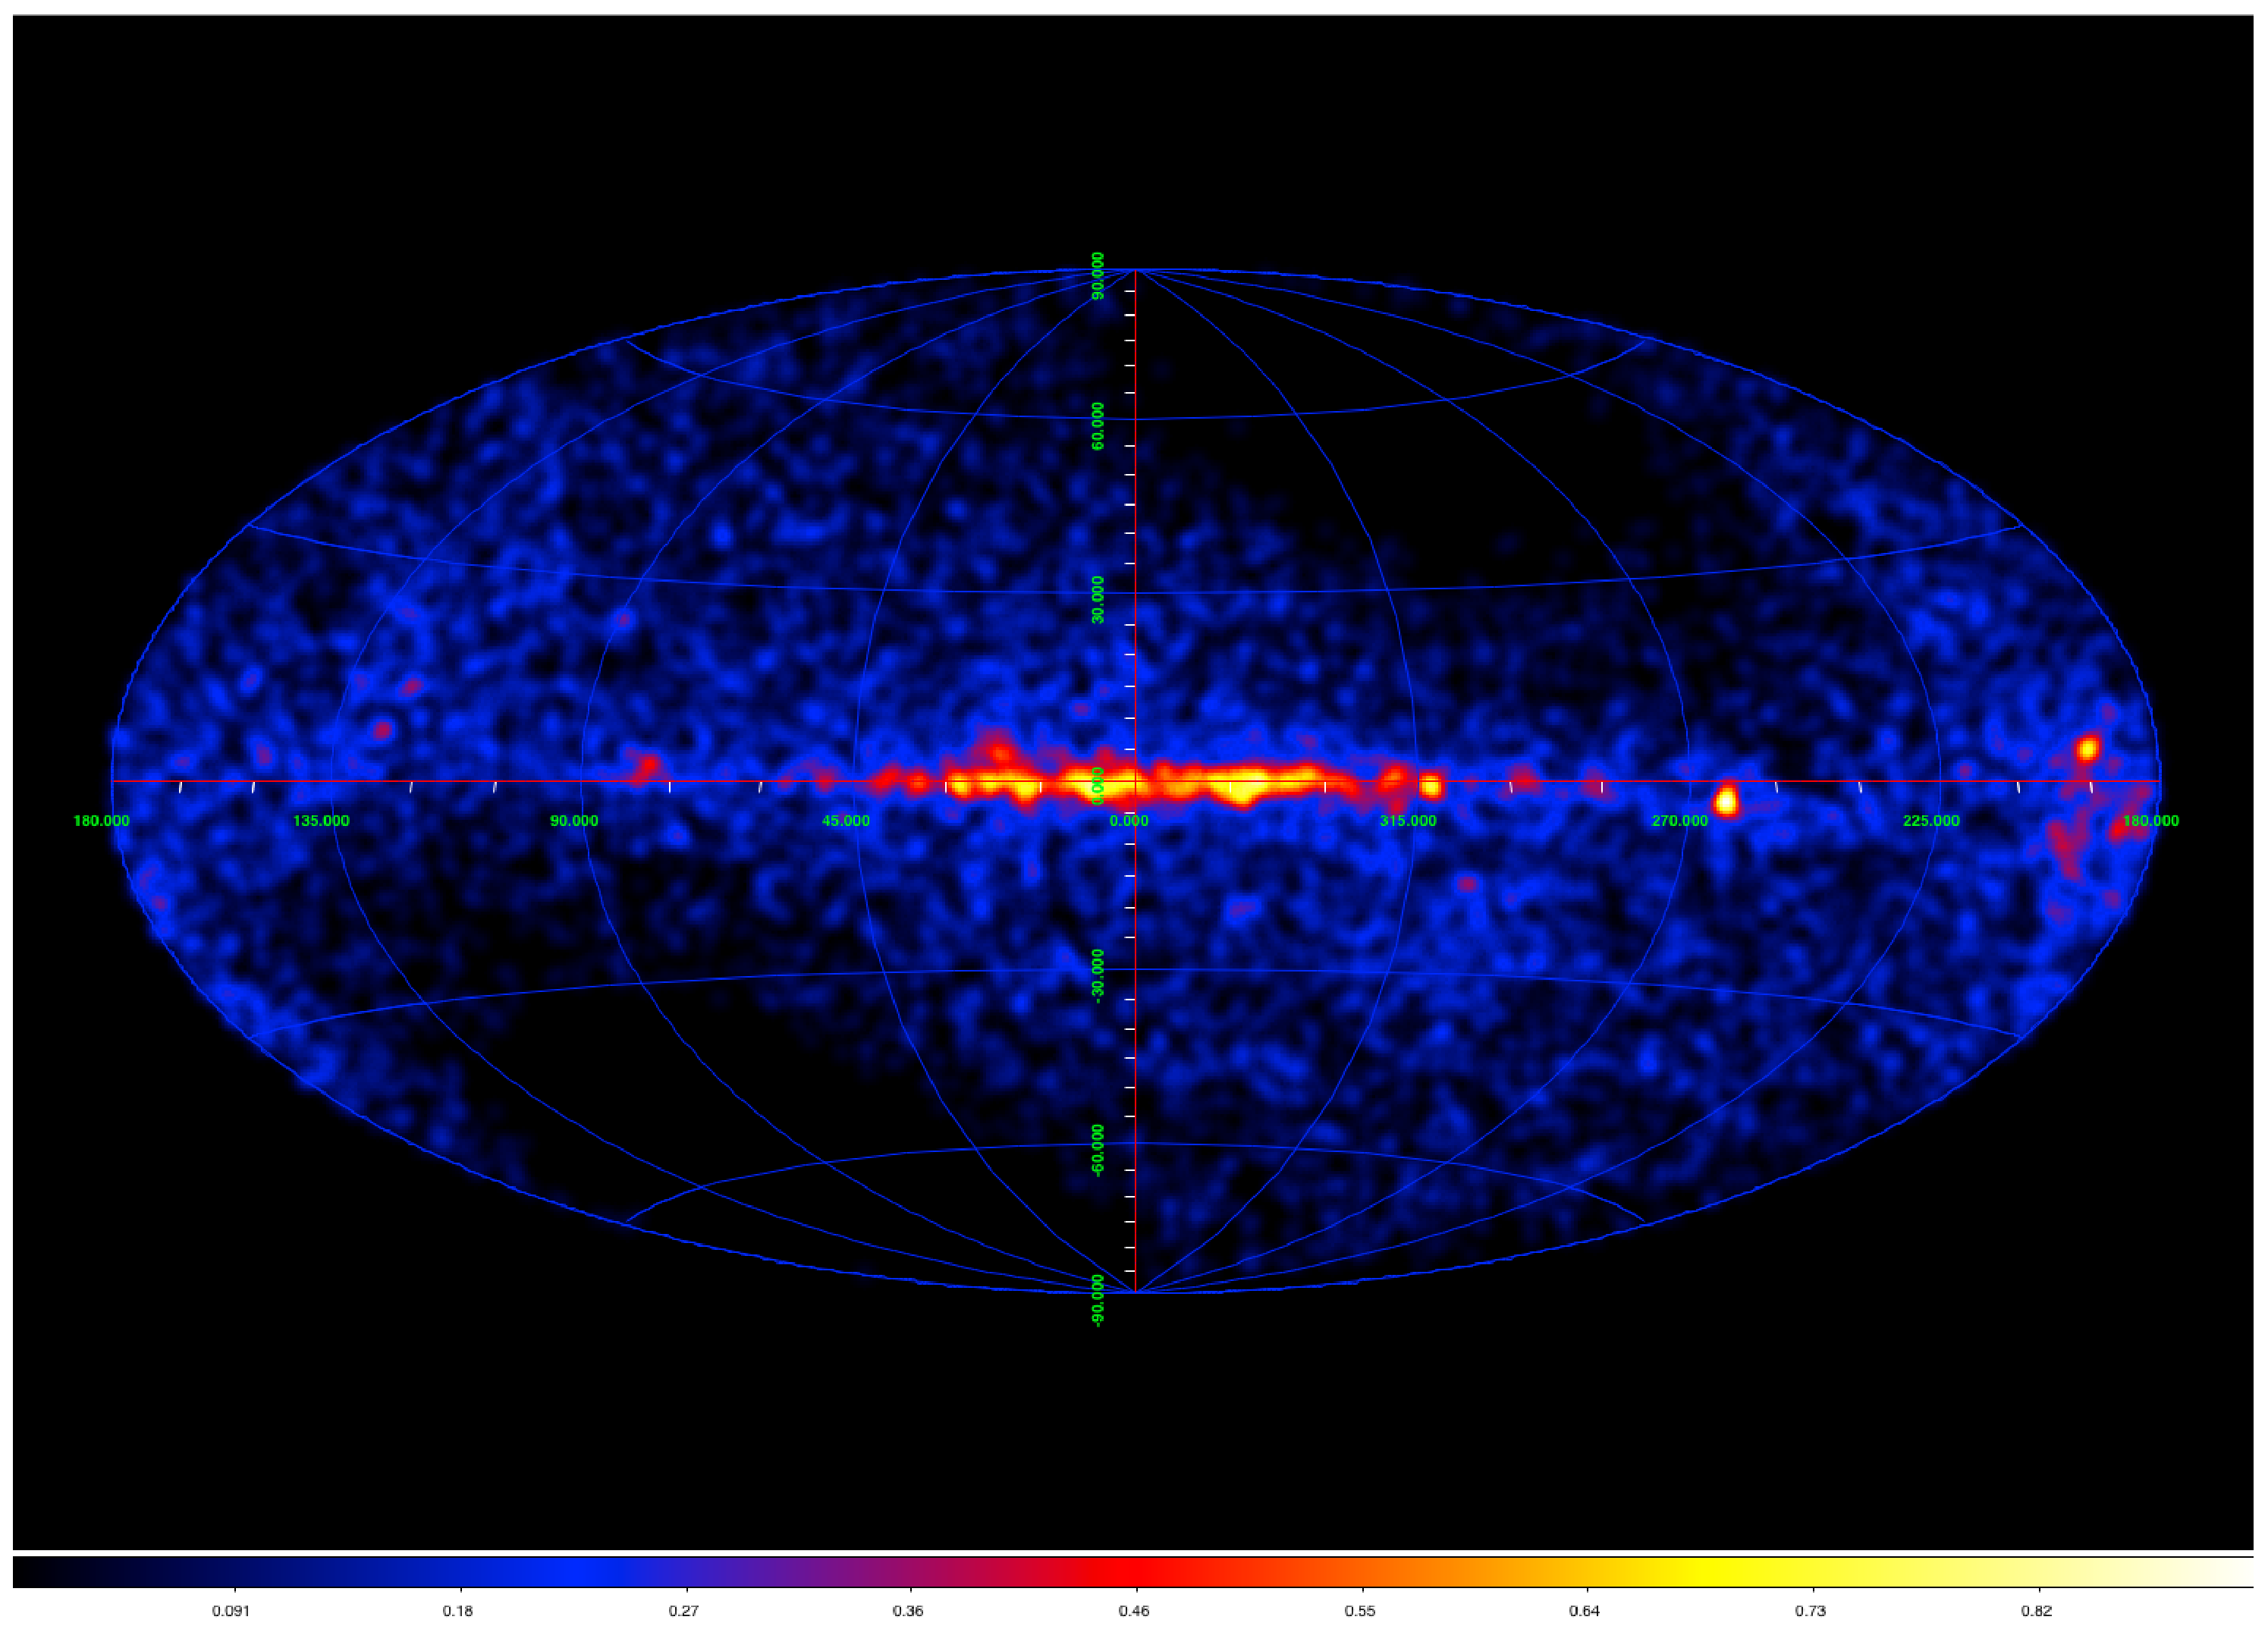
\includegraphics[width=0.75\textwidth]{part10/Bulgarelli_O05/O.05_1c.eps}
\caption{An example of a two-day counts map of \ssindex{observatories!space-based!AGILE}AGILE-\ssindex{instruments!individual!GRID}GRID showing the entire sky in spinning mode in 2012 Oct. The science monitoring system analyzes the entire sky for each orbit, taking into account the regions with low exposure level.} \label{fig_fov}
\end{figure}

\section{The Workflow}

The \ssindex{observatories!space-based!AGILE}AGILE data are down-linked approximately every orbit and sent to the \ssindex{data centers!AGILE Data Center (ADC)}AGILE Data Center (ADC), which is part of the \ssindex{data centers!ASI Science Data Center (ASDC)}ASI Science Data Center (ASDC) for data reduction, scientific processing, and archiving. The \ssindex{data centers!ASI Science Data Center (ASDC)}ASDC then forwards the \ssindex{observatories!space-based!AGILE}AGILE data to the AGILE team local sites where a quick look analysis is performed.

The overall science monitoring alert system of \ssindex{observatories!space-based!AGILE}AGILE is computed by two independent \ssindex{data!pipelines!reduction}pipelines that process the data with different data quality results. The INAF/ IASF Bologna \ssindex{data!pipelines!reduction}pipeline processes the data in the fastest possible way, loosing the tail of the data acquired during an \ssindex{observatories!space-based!AGILE}AGILE orbit (some minutes of acquisition) but it generates alerts within 1.5-2 hours from the time of the last \ssindex{instruments!individual!GRID}GRID event acquired in orbit. The \ssindex{data centers!ASI Science Data Center (ASDC)}ASDC \ssindex{data!pipelines!reduction}pipeline is more accurate because all events are considered during the analysis but the alerts are generated 3-3.5 hours after acquisition.

The description of the software and \ssindex{computers!hardware}hardware data flow is reported in \citep{2009ASPC..411..362B}. The data is analyzed each orbit (when is received) and this produces a sliding window in the generated \ssindex{classification!light curves}light curves of \ssindex{astronomy!gamma-ray}$\gamma$-ray sources (see Figure~\ref{fig_crab}). The selection of candidate flares is performed by two independent methods: (1) with a blind search method called spotfinder and (2) using a list of known sources from different source catalogs. At the end we obtain a list of candidate flares with its related \ssindex{statistical analysis}statistical significance. For a subclass of selected candidate flares with $\sqrt(T_s) \ge 4.5$ an alert is generated and sent via SMS and e-mail.

During the daily monitoring two people are involved in checking the alerts generated by science alert monitoring, one from the AGILE Team (the institutes involved are INAF IASF Bologna, Milan, Palermo, IAPS Rome and INFN Trieste) and one from \ssindex{data centers!ASI Science Data Center (ASDC)}ASDC. The alerts generated by the  IASF Bologna \ssindex{data!pipelines!reduction}pipeline are cross-checked with alerts generated by the \ssindex{data centers!ASI Science Data Center (ASDC)}ASDC \ssindex{data!pipelines!reduction}pipeline. For the most interesting candidate flares, a manual analysis is performed; the detections that survive to this manual check and are above a well defined threshold are taken into consideration for an Astronomical Telegram. Usually we use $\sqrt(T_s) \ge 5$, but when there is an evidence of activity from other wavelengths, a lower significance level is considered. In addition an \ssindex{computing!mobile!iPhone}iPhone \ssindex{computing!mobile!iOS}iOS App has been developed by the AGILE Team at INAF/IASF Bologna. This App is divided into a public section with news, gallery of images, and scientific results and a private, password protected section, where the latest analyzed data are shown to the AGILE Team in an effective way, including the sky maps with the possibility of zooming the maps.
      
      
\section{The Crab Flare Case}

In this case, a maximum likelihood analysis determined that the Crab has a persistent flux of F = $(2.2 +/- 0.1) \cdot 10^{-6} \; ph \; cm^{-2} \; s^{-1}$ for $E > 100$ MeV at a significance of $\sqrt(T_s) = 30.0$ with data from 2007 Jul - 2009 Oct, taking into account the diffuse \ssindex{astronomy!gamma-ray}gamma-ray background with\ssindex{astronomy!Galactic} Galactic and isotropic components, and is obtained considering all nearby sources with a fixed flux. Figure~\ref{fig_crab} reports the sliding light curve of the  2010 Sep Crab flare as seen bythe  \ssindex{observatories!space-based!AGILE}AGILE science monitoring system running at INAF/IASF Bologna. The first alert about the Crab with a flux level that exceed $1-\sigma$ mean flux level (1.a in Figure~\ref{fig_crab}) was received at 2010/09/20 02:04:04 UTC (the yellow arrow 1.b in Figure~\ref{fig_crab} reports the alert generation). The Crab nebula reaches its maximum flux in \ssindex{observatories!space-based!AGILE}AGILE data (see 2.a in Figure~\ref{fig_crab}) between 2010/09/19 01:54:43 UTC and 2010/09/20 23:47:51 in the continuous integration procedure with two days integration time. The alert was generated via email and SMS at 2010/09/21 02:00:54 UTC (see red arrow 2.b in Figure~\ref{fig_crab}), about two hours after the maximum of the physical phenomena. The ATel 2855 \citep{Tavani:ATEL} was posted at 2010-09-22 14:45:00 UTC.
      
The main advantage  of this approach is that the AGILE Team was alerted about the Crab flaring activities at the beginning of the flare itself and thanks to the continuous integration time performed by science alert monitoring the AGILE Team was able to follow the evolution of the overall flaring phenomena in near real-time, providing a fast communication via Astronomical Telegram, enabling other observatories to follow the astrophysical phenomena during its evolution.
      
\begin{figure}[t]
\centering
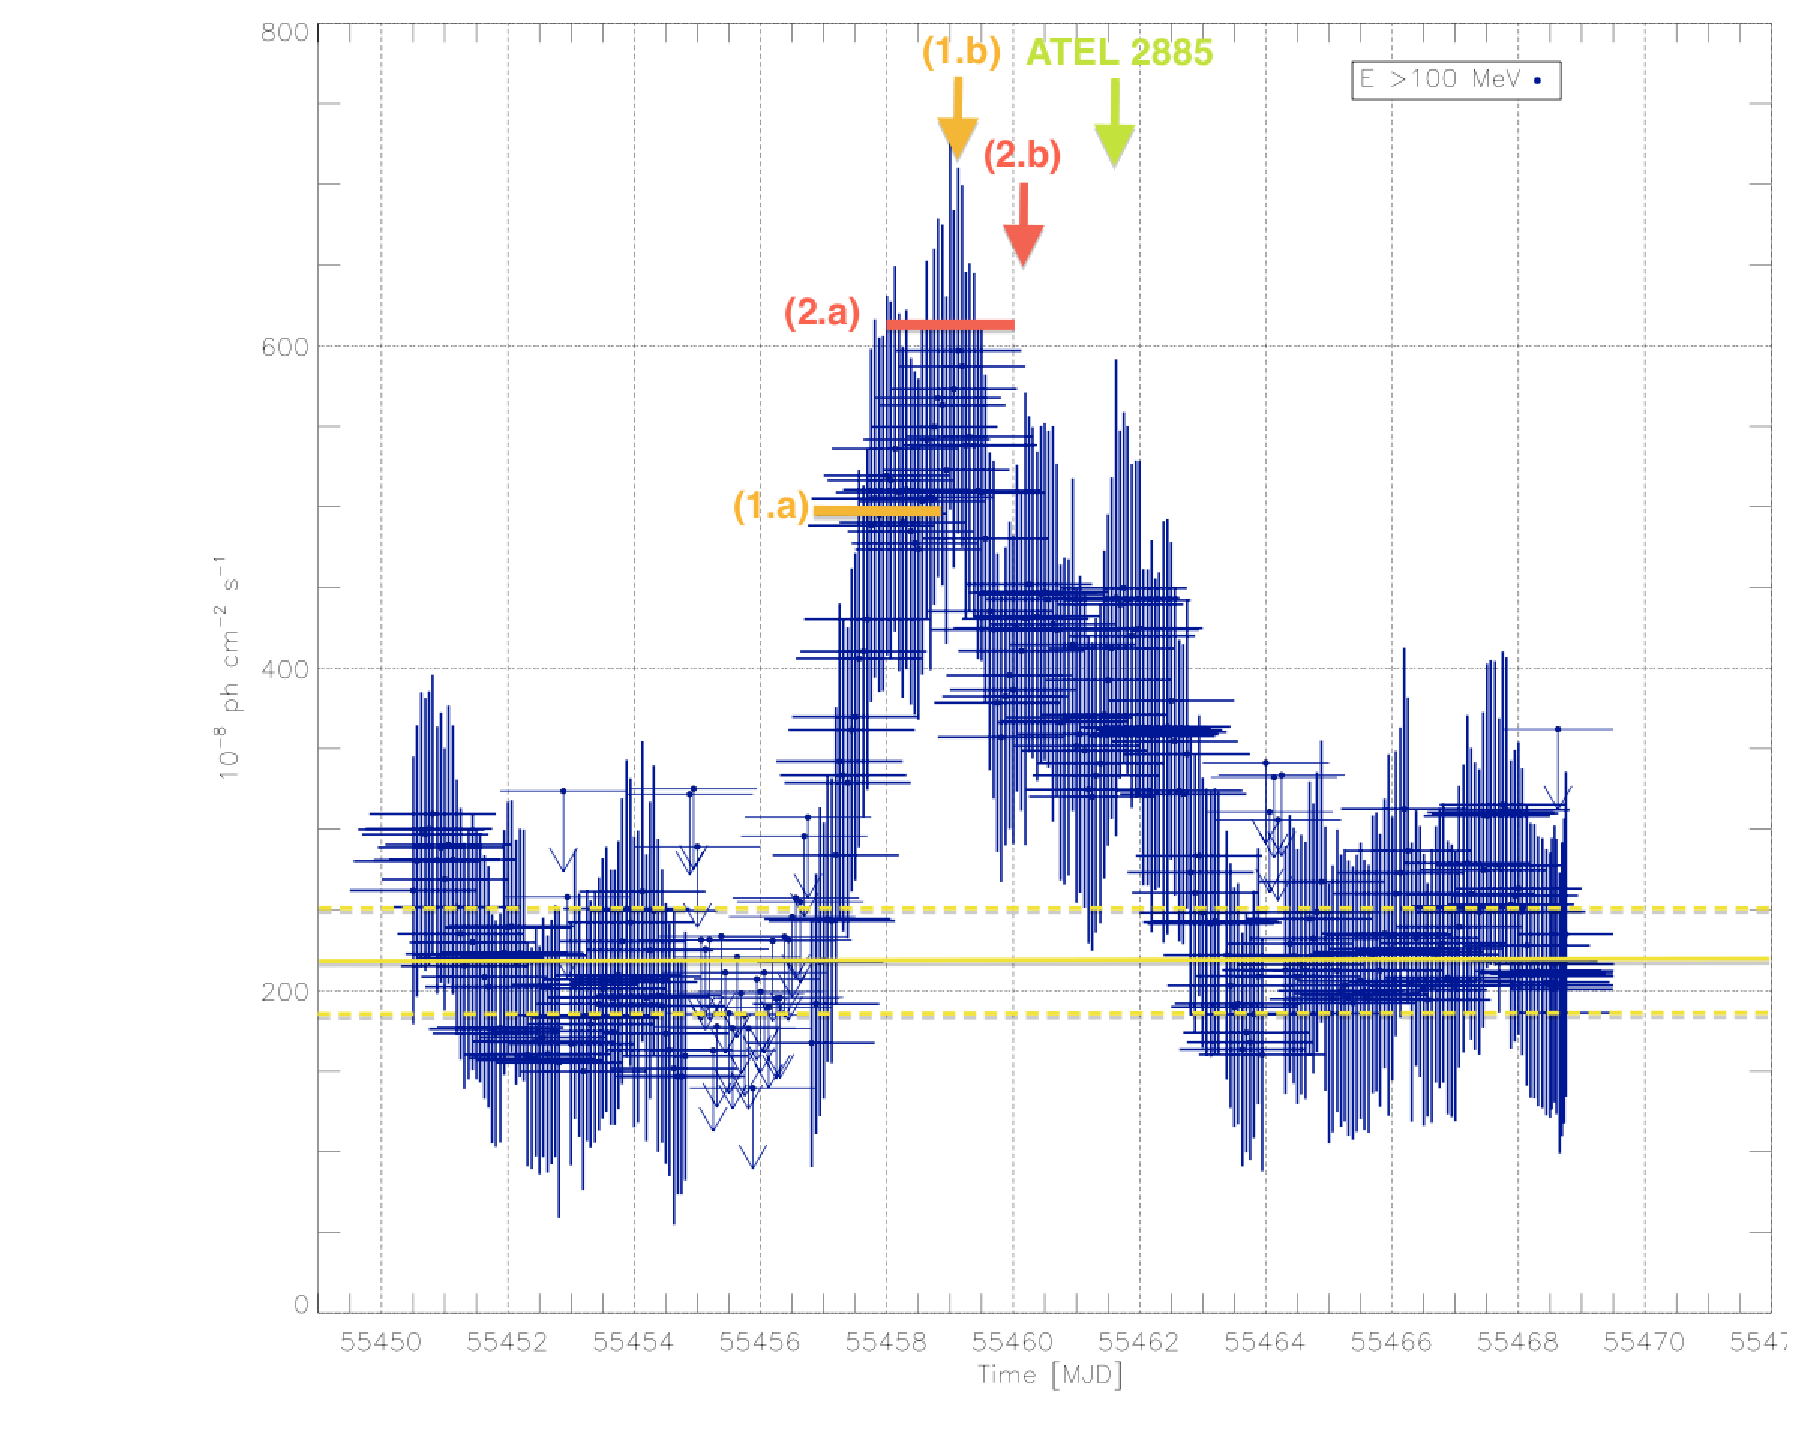
\includegraphics[width=0.75\textwidth]{part10/Bulgarelli_O05/O.05_2.eps}
\caption{The 1.5 hours sliding light curve (2-days integration time) of the September 2010 Crab flare as seen by \ssindex{observatories!space-based!AGILE}AGILE science monitoring system. Errors are $1-\sigma$, and time is given in MJD. The yellow lines show the average Crab flux and the $3-\sigma$ uncertainty range. 1.a and 1.b (in orange) are respectively the detected flux and the time of the alert generation by science monitoring systems when the Crab nebula reached a flux level that exceed $1-\sigma$ the mean flux level; 2.a and 2.b (in red) are related to the reached maximum flux level. The green arrow indicates when the Astronomical Telegram was posted.} \label{fig_crab}
\end{figure}

\section{Conclusion}

The fast data processing and alert generation of INAF/IASF Bologna \ssindex{data!pipelines!reduction}pipeline that maximize the fast data processing with respect to the data quality and the availability of two independent science alert \ssindex{data!pipelines!reduction}pipelines is one of the key factors for the success of the \ssindex{observatories!space-based!AGILE}AGILE mission. The effectiveness of the science alert monitoring system is demonstrated on a daily basis and by the great number of ATel published by AGILE Team; very important discoveries were started by this monitoring system, first of all, the discovery of the Crab flares that earned the 2012 Bruno Rossi prize for Marco Tavani and AGILE Team. This system detects unexpected flaring astrophysical events with a very fast reaction time; this allows an effective follow-up of flaring sources enabling \ssindex{observatories!space-based!AGILE}AGILE to maximize the scientific return in the field of short-timescale phenomenology.

\acknowledgements The \ssindex{observatories!space-based!AGILE}AGILE Mission is funded by the Italian Space Agency (ASI) with scientific and programmatic participation by the Italian Institute of Astrophysics (INAF) and the Italian Institute of Nuclear Physics (INFN). 

\bibliographystyle{asp2010}
\bibliography{editor}
